% Options for packages loaded elsewhere
% Options for packages loaded elsewhere
\PassOptionsToPackage{unicode}{hyperref}
\PassOptionsToPackage{hyphens}{url}
\PassOptionsToPackage{dvipsnames,svgnames,x11names}{xcolor}
%
\documentclass[
  letterpaper,
  DIV=11,
  numbers=noendperiod]{scrartcl}
\usepackage{xcolor}
\usepackage{amsmath,amssymb}
\setcounter{secnumdepth}{-\maxdimen} % remove section numbering
\usepackage{iftex}
\ifPDFTeX
  \usepackage[T1]{fontenc}
  \usepackage[utf8]{inputenc}
  \usepackage{textcomp} % provide euro and other symbols
\else % if luatex or xetex
  \usepackage{unicode-math} % this also loads fontspec
  \defaultfontfeatures{Scale=MatchLowercase}
  \defaultfontfeatures[\rmfamily]{Ligatures=TeX,Scale=1}
\fi
\usepackage{lmodern}
\ifPDFTeX\else
  % xetex/luatex font selection
\fi
% Use upquote if available, for straight quotes in verbatim environments
\IfFileExists{upquote.sty}{\usepackage{upquote}}{}
\IfFileExists{microtype.sty}{% use microtype if available
  \usepackage[]{microtype}
  \UseMicrotypeSet[protrusion]{basicmath} % disable protrusion for tt fonts
}{}
\makeatletter
\@ifundefined{KOMAClassName}{% if non-KOMA class
  \IfFileExists{parskip.sty}{%
    \usepackage{parskip}
  }{% else
    \setlength{\parindent}{0pt}
    \setlength{\parskip}{6pt plus 2pt minus 1pt}}
}{% if KOMA class
  \KOMAoptions{parskip=half}}
\makeatother
% Make \paragraph and \subparagraph free-standing
\makeatletter
\ifx\paragraph\undefined\else
  \let\oldparagraph\paragraph
  \renewcommand{\paragraph}{
    \@ifstar
      \xxxParagraphStar
      \xxxParagraphNoStar
  }
  \newcommand{\xxxParagraphStar}[1]{\oldparagraph*{#1}\mbox{}}
  \newcommand{\xxxParagraphNoStar}[1]{\oldparagraph{#1}\mbox{}}
\fi
\ifx\subparagraph\undefined\else
  \let\oldsubparagraph\subparagraph
  \renewcommand{\subparagraph}{
    \@ifstar
      \xxxSubParagraphStar
      \xxxSubParagraphNoStar
  }
  \newcommand{\xxxSubParagraphStar}[1]{\oldsubparagraph*{#1}\mbox{}}
  \newcommand{\xxxSubParagraphNoStar}[1]{\oldsubparagraph{#1}\mbox{}}
\fi
\makeatother


\usepackage{longtable,booktabs,array}
\newcounter{none} % for unnumbered tables
\usepackage{calc} % for calculating minipage widths
% Correct order of tables after \paragraph or \subparagraph
\usepackage{etoolbox}
\makeatletter
\patchcmd\longtable{\par}{\if@noskipsec\mbox{}\fi\par}{}{}
\makeatother
% Allow footnotes in longtable head/foot
\IfFileExists{footnotehyper.sty}{\usepackage{footnotehyper}}{\usepackage{footnote}}
\makesavenoteenv{longtable}
\usepackage{graphicx}
\makeatletter
\newsavebox\pandoc@box
\newcommand*\pandocbounded[1]{% scales image to fit in text height/width
  \sbox\pandoc@box{#1}%
  \Gscale@div\@tempa{\textheight}{\dimexpr\ht\pandoc@box+\dp\pandoc@box\relax}%
  \Gscale@div\@tempb{\linewidth}{\wd\pandoc@box}%
  \ifdim\@tempb\p@<\@tempa\p@\let\@tempa\@tempb\fi% select the smaller of both
  \ifdim\@tempa\p@<\p@\scalebox{\@tempa}{\usebox\pandoc@box}%
  \else\usebox{\pandoc@box}%
  \fi%
}
% Set default figure placement to htbp
\def\fps@figure{htbp}
\makeatother


% definitions for citeproc citations
\NewDocumentCommand\citeproctext{}{}
\NewDocumentCommand\citeproc{mm}{%
  \begingroup\def\citeproctext{#2}\cite{#1}\endgroup}
\makeatletter
 % allow citations to break across lines
 \let\@cite@ofmt\@firstofone
 % avoid brackets around text for \cite:
 \def\@biblabel#1{}
 \def\@cite#1#2{{#1\if@tempswa , #2\fi}}
\makeatother
\newlength{\cslhangindent}
\setlength{\cslhangindent}{1.5em}
\newlength{\csllabelwidth}
\setlength{\csllabelwidth}{3em}
\newenvironment{CSLReferences}[2] % #1 hanging-indent, #2 entry-spacing
 {\begin{list}{}{%
  \setlength{\itemindent}{0pt}
  \setlength{\leftmargin}{0pt}
  \setlength{\parsep}{0pt}
  % turn on hanging indent if param 1 is 1
  \ifodd #1
   \setlength{\leftmargin}{\cslhangindent}
   \setlength{\itemindent}{-1\cslhangindent}
  \fi
  % set entry spacing
  \setlength{\itemsep}{#2\baselineskip}}}
 {\end{list}}
\usepackage{calc}
\newcommand{\CSLBlock}[1]{\hfill\break\parbox[t]{\linewidth}{\strut\ignorespaces#1\strut}}
\newcommand{\CSLLeftMargin}[1]{\parbox[t]{\csllabelwidth}{\strut#1\strut}}
\newcommand{\CSLRightInline}[1]{\parbox[t]{\linewidth - \csllabelwidth}{\strut#1\strut}}
\newcommand{\CSLIndent}[1]{\hspace{\cslhangindent}#1}



\setlength{\emergencystretch}{3em} % prevent overfull lines

\providecommand{\tightlist}{%
  \setlength{\itemsep}{0pt}\setlength{\parskip}{0pt}}



 


\usepackage{setspace}
\onehalfspacing

\usepackage[pagewise]{lineno}
\linenumbers

\usepackage{xcolor}
\usepackage{afterpage}
\usepackage{eso-pic}
\definecolor{thesiscream}{RGB}{255, 252, 240}
\definecolor{thesissand}{RGB}{232, 212, 162}
\pagecolor{thesiscream}
\KOMAoption{captions}{tableheading}
\makeatletter
\@ifpackageloaded{caption}{}{\usepackage{caption}}
\AtBeginDocument{%
\ifdefined\contentsname
  \renewcommand*\contentsname{Table of contents}
\else
  \newcommand\contentsname{Table of contents}
\fi
\ifdefined\listfigurename
  \renewcommand*\listfigurename{List of Figures}
\else
  \newcommand\listfigurename{List of Figures}
\fi
\ifdefined\listtablename
  \renewcommand*\listtablename{List of Tables}
\else
  \newcommand\listtablename{List of Tables}
\fi
\ifdefined\figurename
  \renewcommand*\figurename{Figure}
\else
  \newcommand\figurename{Figure}
\fi
\ifdefined\tablename
  \renewcommand*\tablename{Table}
\else
  \newcommand\tablename{Table}
\fi
}
\@ifpackageloaded{float}{}{\usepackage{float}}
\floatstyle{ruled}
\@ifundefined{c@chapter}{\newfloat{codelisting}{h}{lop}}{\newfloat{codelisting}{h}{lop}[chapter]}
\floatname{codelisting}{Listing}
\newcommand*\listoflistings{\listof{codelisting}{List of Listings}}
\makeatother
\makeatletter
\makeatother
\makeatletter
\@ifpackageloaded{caption}{}{\usepackage{caption}}
\@ifpackageloaded{subcaption}{}{\usepackage{subcaption}}
\makeatother
\usepackage{bookmark}
\IfFileExists{xurl.sty}{\usepackage{xurl}}{} % add URL line breaks if available
\urlstyle{same}
\hypersetup{
  pdftitle={Fear of the new: a predatory invader provokes stronger non-consumptive effects on a keystone native prey than a native predator},
  pdfauthor={Olivier V. Raven; Calum MacNeil; Finnbar Lee; Robin Holmes; Ian A. Kusabs; Francis J. Burdon; Deniz Özkundakci},
  pdfkeywords={Non-consumptive effects, Crayfish, Kōura, Brown bullhead
catfish, Antipredator behaviour},
  colorlinks=true,
  linkcolor={blue},
  filecolor={Maroon},
  citecolor={Blue},
  urlcolor={Blue},
  pdfcreator={LaTeX via pandoc}}


\title{Fear of the new: a predatory invader provokes stronger
non-consumptive effects on a keystone native prey than a native
predator}
\author{Olivier V. Raven \and Calum MacNeil \and Finnbar Lee \and Robin
Holmes \and Ian A. Kusabs \and Francis J. Burdon \and Deniz Özkundakci}
\date{2026-07-07}
\begin{document}
\maketitle
\begin{abstract}
The non-consumptive effects (NCEs) of predators on prey result in costly
antipredator behaviours, including increased refuge use and reduced
foraging. NCEs significantly influence prey population dynamics,
community interactions, and affect ecosystem functioning, particularly
when the prey are keystone species. In Aotearoa-New Zealand, the native
freshwater crayfish kōura (\emph{Paranephrops planifrons}) is a keystone
species with an important functional role affecting sediment
bioturbation, nutrient cycling, and benthic community structure. Kōura
are preyed upon by multiple predators including native longfin eel
(\emph{Anguilla dieffenbachii}) and invasive brown bullhead catfish
(\emph{Ameiurus nebulosus}). Under laboratory conditions, we tested
whether visual and chemical cues from these two predators induced
different refuge-seeking and feeding behaviour responses by kōura.
Predator presence produced in the dark a NCE on refuge use, with kōura
exposed to catfish showing significantly greater refuge-seeking
behaviour than those exposed to eels. This result is consistent with the
generalisation theory triggered by unfamiliar predator cues rather than
classic prey naivety. Our study indicates catfish incursions may provoke
a greater NCE on kōura behaviours than resident eels. As catfish range
expansion continues, these NCEs may represent an ecologically
significant and underappreciated threat to kōura populations,
compounding the direct predation pressure already documented for this
invader.
\end{abstract}

\renewcommand*\contentsname{Table of contents}
{
\setcounter{tocdepth}{3}
\tableofcontents
}

\thispagestyle{empty}
\AddToShipoutPictureBG*{\AtPageUpperLeft{\includegraphics[width=\paperwidth,height=\paperheight]{images/ch2_cover.jpg}}}
\null
\newpage
\pagecolor{thesissand}
\vspace{1cm}
\begin{center}
\textit{How do native and non-native predators differentially influence antipredator behaviour and refuge use in kōura?}
\end{center}
\afterpage{\pagecolor{thesiscream}}

\subsection{Introduction}\label{introduction}

Biological invasions can have profound impacts on invaded ecosystems,
particularly through the introduction of novel predators that prey upon
naïve native species lacking coevolved defence mechanisms
(\citeproc{ref-Doherty2016}{Doherty et al. 2016}). Native prey may be
naïve not just to a specific invader, but to entire functional groups of
predators, making them especially vulnerable to direct predation when an
invasion introduces a predator type entirely absent from their
evolutionary history (\citeproc{ref-Sih2010}{Sih et al. 2010};
\citeproc{ref-Carthey2014}{Carthey and Banks 2014}). In addition to
these consumptive effects, native prey may exhibit heightened fear
responses to invasive predators, leading to the development of
anti-predator behaviours such as increased refuge use and avoidance of
open habitats (\citeproc{ref-Kindlinger2017}{Kindinger and Albins
2017}). These behavioural changes, termed non-consumptive effects
(NCEs), can substantially influence population dynamics by reducing
foraging activity, growth, and reproductive output
(\citeproc{ref-Preisser2005}{Preisser et al. 2005}). In contrast, native
predators generally elicit different responses because prey and
predators have coevolved, resulting in behavioural and physiological
adaptations that stabilise predator--prey interactions
(\citeproc{ref-Abrams2000}{Abrams 2000}).

Chemical signals (kairomones) are a key component of NCEs
(\citeproc{ref-Kasumyan2022}{Kasumyan 2022}). Freshwater crayfish
release and detect kairomones to help navigate aquatic environments and
mediate interactions with predatory fish (\citeproc{ref-Blake1993}{Blake
and Hart 1993}; \citeproc{ref-Bronmark2012}{Brönmark and Hansson 2012};
\citeproc{ref-Wood2020b}{Wood and Moore 2020a}). Kairomones carry
signals via excreta, mucus, or skin, that crayfish use to detect
predators (\citeproc{ref-Appelberg1993}{Appelberg et al. 1993}).
Crayfish respond more strongly to signals from predators that have
consumed conspecifics and to alarm cues released when conspecifics are
injured or killed (\citeproc{ref-Gherardi2011}{Gherardi et al. 2011};
\citeproc{ref-Beattie2018}{Beattie and Moore 2018}). The NCEs due to
kairomone detection include reduced growth, reduced activity levels
(\citeproc{ref-Adams2007}{Adams 2007};
\citeproc{ref-RambergPihl2020}{Ramberg-Pihl and Yurewicz 2020}), and
altered social dynamics like the use of refuge spaces
(\citeproc{ref-Driscoll2020}{Driscoll et al. 2020}). Non-predatory fish
can also trigger behaviour changes, likely through an increased
awareness of potential risk (\citeproc{ref-Nystrom2005}{Nyström 2005}).
However, the strength of these responses depends on prior experience as
wild-caught individual crayfish show stronger antipredator responses
than farmed conspecifics naïve to predators
(\citeproc{ref-Martin2014}{Martin 2014}), indicating that both learned
behavior and evolutionary history shape kairomone detection.

In Aotearoa-New Zealand (hereafter Aotearoa), the endemic northern
freshwater crayfish \emph{Paranephrops planifrons} (White, 1842) is a
keystone species impacted by non-native species. This crayfish species
is commonly known as kōura and is a taonga (culturally treasured)
species for Māori, the indigenous people of Aotearoa, with strong
cultural values as a food resource (\citeproc{ref-Kusabs2009}{Kusabs and
Quinn 2009}). Ecologically, kōura play a critical role as ecosystem
engineers through their effects on sediment dynamics, nutrient cycling,
and benthic community structure (\citeproc{ref-Collier1997}{Collier et
al. 1997}; \citeproc{ref-Parkyn2001}{Parkyn et al. 2001};
\citeproc{ref-Usio2004}{Usio and Townsend 2004}). Currently, kōura are
threatened by multiple stressors, including climate change,
water-quality degradation and invasive species, contributing to
widespread population declines (\citeproc{ref-Lee2025}{Lee et al. 2025};
\citeproc{ref-Kusabs2026}{Kusabs et al. 2026}).

Kōura have a long coevolutionary history with the native longfin eel
(\emph{Anguilla dieffenbachii}) (hereafter eel) and shortfin eel
(\emph{A. australis}) in Aotearoa (\citeproc{ref-Brown2009}{Brown 2009};
\citeproc{ref-MacNeil2025}{MacNeil et al. 2025}). Reflecting this
coevolutionary history, kōura can respond more strongly to eel
kairomones than to those of introduced non-native brown trout
(\emph{Salmo trutta}), even when sourced from streams where both
predators were present (\citeproc{ref-Shave1994}{Shave et al. 1994}).
Shave et al. (\citeproc{ref-Shave1994}{1994}) suggest that kōura
predator recognition is a fixed behavioural trait shaped by coevolution.
An invasive fish species that threatens kōura is the brown bullhead
catfish (\emph{Ameiurus nebulosus}) (hereafter catfish). Catfish were
introduced to Aotearoa in 1877, and the invasive species has since
spread to multiple lakes and rivers in the North Island
(\citeproc{ref-McDowall1990}{McDowall 1990};
\citeproc{ref-Barnes2003}{Barnes and Hicks 2003};
\citeproc{ref-Dedual2019}{Dedual 2019}). For example, in 2016/18, the
presence of catfish was confirmed in two large volcanic lakes, Lakes
Rotoiti and Rotorua in the Bay of Plenty region, which have historically
contained large populations of kōura (\citeproc{ref-Francis2019}{Francis
2019}; \citeproc{ref-Lee2025}{Lee et al. 2025}). Catfish are highly
tolerant of a wide range of environmental conditions
(\citeproc{ref-Scott1973}{Scott and Crossman 1973};
\citeproc{ref-Lee2025}{Lee et al. 2025}) and their broad gape and
opportunistic feeding behaviour enable the consumption of a wide variety
of aquatic prey (\citeproc{ref-Scott1973}{Scott and Crossman 1973};
\citeproc{ref-Dedual2019}{Dedual 2019}). Given Aotearoa lacks native
Siluriformes, the recent and ongoing spread of catfish into North Island
waterways represents a truly novel predation threat to which kōura may
lack adequate behavioural or sensory adaptations to respond.

In this study, we used controlled laboratory experiments to test whether
the presence of a novel and native predator induced differences in kōura
NCEs, specifically refuge-seeking and feeding behaviours. Our
experiments tested the following two hypotheses regarding kōura
behavioural responses to predator cues: 1) Kōura would show less
shelter-seeking behaviour when presented with catfish compared to eels,
due to naivety towards a novel predator
(\citeproc{ref-Carthey2014}{Carthey and Banks 2014}); or 2) kōura would
respond more strongly to unfamiliar catfish cues than to the native eel,
consistent with a generalised fear response to a novel predator type
(\citeproc{ref-Sih2023}{Sih et al. 2023}). Further, we expected that
light regime would have an influence on shelter seeking behaviour, as
kōura, like many crayfish, are primarily nocturnal
(\citeproc{ref-Devcich1979}{Devcich 1979};
\citeproc{ref-Johnson2014}{Johnson et al. 2014}). We also predicted that
kōura feeding rates would follow the patterns hypothesized above and
either be more in the presence of catfish than eels, reflecting stronger
antipredator responses to the native predator, or reduced in the
presence of the unfamiliar invasive predator, reflecting a generalised
fear response to the novel predator. Overall, the refuge-use and feeding
experiment aimed to improve understanding of the behavioural mechanisms
underlying kōura vulnerability to invasive catfish, and how these
responses may differ, and add to, those displayed in the presence of
native predators such as eels.

\subsection{Materials and Methods}\label{materials-and-methods}

\subsubsection{Animal collection and
preparation}\label{animal-collection-and-preparation}

In mid-August 2025, 92 kōura were sourced from two catfish-free lakes,
Ōkāreka and Tikitapu, within the Rotorua Te Arawa Lakes area in the
North Island of Aotearoa. Eels are rare or absent in these lakes
(\citeproc{ref-Martin2007}{Martin et al. 2007}), potentially limiting
the recent coevolutionary history with local kōura populations. However,
eels are a native predator that has a long record of coexistence with
kōura in Aotearoa (\citeproc{ref-McDowall1990}{McDowall 1990};
\citeproc{ref-Feldmann1994}{Feldmann and Pole 1994};
\citeproc{ref-Kaulfuss2018}{Kaulfuss et al. 2018}). In this study our
focus was on the macroevolutionary implications of the native predator
compared to a novel invader, regardless of the local coevolutionary
history. In late September 2025, catfish and eels were sourced from Lake
Rotoroa in Hamilton in the Waikato region of the North Island.
Experiments were conducted at the Aquatic Research Centre of the
University of Waikato. All three species were held separately in holding
tanks and acclimated for a week in the laboratory conditions. These
included a 10:14 light:dark cycle reflecting the seasonal day-length and
dechlorinated tap water with stable temperatures (15.6 °C), pH (8.4) and
dissolved oxygen concentrations (10 mg l⁻¹). These parameters reflect
typical physiochemical conditions in the source lakes. Kōura and fish
were fed every other day with commercial carnivore pellets (Hikari
Tropical, Kyorin Food Industries Ltd., Japan; animal protein 47 \%).
Because kōura are a taonga (treasured) species, permission was obtained
from Te Arawa Lakes Trust and Te Komiti Whakahaere. All experimental
procedures were conducted under University of Waikato animal ethics
committee approval (protocol number: 1232; see Ethical Approval
section).

\subsubsection{Refuge experiment}\label{refuge-experiment}

Prior to the experiments all animals were individually weighed and
measured. Only male kōura were used as male crustaceans are usually the
most bold and aggressive (\citeproc{ref-Stein1976}{Stein and Magnuson
1976}; \citeproc{ref-Figler2005}{Figler et al. 2005}) and restricting
test animals to a single sex allowed a smaller overall number of kōura
to be used. Kōura had a mean (± SD) orbital carapace length (OCL) of
26.0 mm (± 3.08) (18.35-32.95 mm range) and a mean (± SD) wet weight of
11.7 g (± 4.25) (3--23 g range). Catfish ranged in length from 260-267
mm and 2.34--3.16 kg wet weight and eels ranged in wet weight from
2.50-3.52 kg, with both these size ranges being able to consume adult
kōura (\citeproc{ref-Hicks1997}{Hicks 1997};
\citeproc{ref-Barnes2003}{Barnes and Hicks 2003};
\citeproc{ref-Ryan2009}{Ryan 2009}).

Experiments were conducted in 38 L glass tanks (600 × 200 × 220 mm) with
each tank having three sides (apart from front of tank) blacked out to
block visual cues from neighbouring tanks. Each tank was divided into
two compartments by a 0.5 mm steel mesh divider, allowing visual and
chemical cues between compartments, while preventing any physical
contact between fish and kōura on either side of the barrier
(Figure~\ref{fig-aquarium-setup}). All tanks were filled with
\textasciitilde26 L dechlorinated tap water and had identical
environmental regimes as previously detailed for acclimatisation tanks,
with water flow provided by an air stone. Each tank housed a single
kōura on one side of the barrier and either a single predator (catfish
or eel) or no predator (control) on the other side. A halved terracotta
pot (90 mm diameter × 90 mm depth) was positioned on the kōura side of
the tank to serve as a potential refuge. To control for potential tank
location or compartment side effects, the position of predator
treatments within the aquaria was systematically rotated between
experimental rounds. The experiment was conducted across eight rounds
(each lasting 5 hours), four rounds under light conditions
(\textasciitilde400 lux, n = 32 kōura: 11 catfish, 11 eel, 10 control)
and four separate rounds with different kōura under dark conditions
(\textasciitilde70 lux, n = 32 kōura: 11 catfish, 11 eel, 10 control).
Observations were made in the dark using red lighting positioned
centrally above the tanks to minimize disturbance, as many aquatic
species have limited sensitivity to red wavelengths and are unlikely to
perceive this part of the spectrum. Following each individual
experimental run, each tank was thoroughly cleaned and refilled with
dechlorinated tap water before reuse. Each individual kōura was only
exposed once to a fish predator and there were no mortalities of kōura
or fish during experiments. All experiments were conducted within a
three-week period during October 2025.

At the beginning of each experiment, an individual kōura was placed in
the middle of the tank compartment containing the refuge. Kōura location
was recorded at 21-time intervals over a 5-hour period, with
observations spaced at progressively longer intervals to capture
immediate behavioural responses at key timepoints (predator introduction
at 60 min, removal at 240 min). The 0-minute recording was the
individual's initial immediate location after its addition to the tank.
Kōura location was recorded as either refuge (the animal was using the
refuge, being inside it or immediately behind it and touching it) or
non-refuge/ in the open (any other location in the tank where the animal
was not in the refuge or touching the refuge). The control tanks had no
fish added but at 60 minutes and again at 240 minutes, the water in the
`predator' compartment was mechanically disturbed by agitating the water
with a small hand net for approximately 30 seconds. This was to simulate
the disturbance time associated with adding and removing fish in the
other treatments with the same size hand net. At the end of each
experiment, the kōura was removed after the final 300-minute
observation.

\subsubsection{Feeding experiment}\label{feeding-experiment}

Experiments were conducted in glass tanks (320 × 170 × 170 mm),
containing 5 L dechlorinated tap water and a halved terracotta pot (90
mm diameter × 90 mm depth). Catfish and eels had been held at the same
density in separate identical holding tanks for a week prior to
experiment. Fish exudates were collected by placing four fish (catfish
or eel) in a 10 L bucket filled with water from the holding tanks for 15
minutes to concentrate the kairomones in the water. For eel and catfish
treatments, 1 L from the buckets was added to each tank already holding
5 L of tap water, and for control an additional 1 L of dechlorinated tap
water was added. Next, 10 Hikari Tropical carnivore pellets were added
to each tank. Experimental trials showed pellets remain intact in tap
water for over 24 hours. In three rounds, a total of 46 male kōura were
measured and weighed. Their mean (± SD) OCL was 27.93 mm (± 4.80), with
a range of 20.48 to 40.88 mm, and the mean (± SD) wet weight of 15.83 g
(± 8.99), ranging from 6.00 to 42.00 g. Each kōura was then placed
individually in a tank. To investigate how starvation period influenced
feeding motivation, each round kōura were starved for different periods
(either 0, 3 or 4 days) prior to the feeding experiment. After 0 days
starvation, 14 kōura were exposed to eel water (n = 4), catfish water (n
= 6) or control water (n = 4). After 3 days starvation, 16 kōura were
exposed to eel water (n = 6), catfish water (n = 5) or control water (n
= 5). After 4 days starvation, 16 kōura were exposed to eel water (n =
5), catfish water (n = 5) or control water (n = 6). After 24 hours, when
each experiment was terminated, the number of pellets eaten (to the
nearest quarter pellet) was counted and the feeding rate (pellets eaten
per gram of wet weight (WW) of kōura) calculated.

\subsubsection{Data analysis}\label{data-analysis}

To analyse kōura refuge use, beta-binomial generalized linear
mixed-effects models (GLMMs) were fitted using the glmmTMB package in R
(\citeproc{ref-Brooks2017}{Brooks et al. 2017};
\citeproc{ref-RCoreTeam2025}{R Core Team 2025}). To address potential
non-independence of repeated observations within tanks, raw observations
were first aggregated into three experimental periods (before, during,
and after predator introduction) per individual kōura, with the number
of observations in refuge out of total observations per period used as
the response variable. Treatment (catfish, eel, control) and period
(before, during, after) were included as fixed effects, and tank and
experimental round as random intercepts. Because light condition and
experimental round were fully confounded by design (rounds 1--4 in
light, rounds 5--8 in darkness), separate analyses were conducted for
each light condition to allow round as a random intercept and to test
whether treatment effects varied under each light condition. A
beta-binomial distribution was used to account for overdispersion in the
binomial proportion data. Model fit was assessed using DHARMa
simulation-based residuals, including tests for overdispersion and
zero-inflation (\citeproc{ref-Hartig2024}{{Hartig et al.} 2024}).
Marginal means and pairwise contrasts between factor levels were
obtained using the emmeans package (\citeproc{ref-Lenth2026}{Lenth et
al. 2026}), with p-values adjusted for multiple comparisons using Sidak
correction. Additionally, a combined GLMM (without round as random
effect) was fitted to test the overall effect of light condition across
all treatments. Spearman rank correlations with Bonferroni-adjusted
p-values were used to investigate potential relationships between kōura
body size (OCL) and overall refuge use (all time intervals combined) in
the three treatments.

Kōura feeding rate was analysed using a linear mixed model with pellets
consumed per gram wet weight as the response variable and starvation
period (0, 3, 4) as a fixed effect, with tank identity as a random
intercept to account for potential tank-level clustering. Because each
starvation period was conducted in a separate experimental round,
starvation period and experimental round were fully confounded by
design. Consequently, round was excluded as a random effect. However,
starvation period was included as a fixed effect to test for differences
in feeding across hunger states, acknowledging that observed effects may
reflect round-specific variation rather than hunger alone. Model
selection using AICc indicated that starvation period alone provided the
best fit, with treatment not improving model fit (delta AICc = 14.38).
Therefore, treatment effects were excluded from the main model and
instead examined separately within each starvation period using
stratified linear models to avoid confounding treatment comparisons with
the starvation-round confounding. Model assumptions were verified using
residual diagnostics (Q-Q plots and residual plots) and testing
normality of residuals using the Shapiro-Wilk test. As residuals at day
0 starvation violated normality assumptions (\emph{p} = 0.011), a
non-parametric Kruskal-Wallis test was executed. Pairwise comparisons
for starvation period were conducted using estimated marginal means with
Sidak adjustment for multiple comparisons.

\subsection{Results}\label{results}

\subsubsection{Refuge experiment}\label{refuge-experiment-1}

The proportion of time kōura spent in refuge varied across treatments,
experimental periods, and light conditions
(Figure~\ref{fig-emmeans-stratified}). Stratified analyses revealed that
treatment effects on refuge use differed between light and dark
conditions. Under dark condition, kōura exposed to catfish used refuge
significantly more than those exposed to eels (\emph{p} = 0.004;
Table~\ref{tbl-emmeans-stratified}), however the control treatment in
the dark was not significant with either the catfish or the eel
treatment (\emph{p} = 0.083, \emph{p} = 0.565). In contrast, under light
conditions, there were no significant differences in refuge use between
the three treatments, but refuge use differed significantly between
experimental periods, with lower refuge use before predator introduction
compared to after predator removal (\emph{p} = 0.021). No significant
period effects were observed in dark conditions. The combined model
showed that light regime had a significant effect on refuge use
(\emph{p} = 0.005), with kōura using refuge more in light than in dark
conditions across all treatments. Overall, under light conditions, the
pattern of refuge use in the control treatment was more similar to the
catfish treatment, whereas under dark conditions it more resembled the
eel treatment (Fig. 3; Table S1). There was also no relationship between
kōura OCL and refuge use in any of the three treatments (rs = -0.09,
\emph{p} = 0.693, rs = 0.09, \emph{p} = 0.680 and rs = 0.16, \emph{p} =
0.494 for catfish, eel and control treatments respectively, all NS).

For all treatments individual kōura were highly variable in their
movement around tanks and use of refuges, even in the time intervals
comprising the first 60 minutes of the experiment, before fish were
introduced. The coefficient of variations (CVs) for kōura refuge use in
the light and the dark before fish introduction were similarly high,
being 60.4 \% and 58.2 \% (both n = 32) respectively, confirming high
baseline variation in kōura refuge use, regardless of treatment type.
Despite this inherent variation in individual kōura behaviour, clear
patterns in kōura refuge use were evident over the course of the
experiment (Figure~\ref{fig-refuge-plot}). Under light conditions, the
control showed the largest overall increase in refuge use (40\% to
82\%), driven primarily by a sharp rise in the `after' period, while the
catfish treatment showed a more sustained increase across all periods
(52\% to 73\%) and the eel treatment the smallest increase (35\% to
53\%). Under dark conditions, the pattern shifted, with the catfish
treatment showing the greatest increase (39\% to 70\%), while the eel
treatment showed a modest and non-sustained increase (27\% to 41\%
during `exposure', returning to 36\% `after'), and the control remained
comparatively low throughout (37\% to 47\%).

\subsubsection{Feeding experiment}\label{feeding-experiment-1}

The linear mixed model showed that starvation period had a significant
effect on kōura feeding rate (3 days: \emph{p} \textless{} 0.001; 4
days: \emph{p} = 0.046; Figure~\ref{fig-feeding-plot};
Table~\ref{tbl-feeding-summary}). Treatment was not included in the main
model following model selection. Stratified analyses revealed no
significant treatment effects across starvation periods. Although
residuals at day 0 violated normality (Shapiro-Wilk \emph{p} = 0.0112),
the non-parametric Kruskal-Wallis test confirmed no treatment effect
(\emph{p} = 0.3165). Starvation days 3 and 4 met normality assumptions
and showed no significant treatment effects (\emph{p} = 0.1495 and
0.1573 respectively). After 4 days starvation, the mean (±SE) kōura
feeding rate (pellets g WW⁻¹) for the control was over two and a half
times that of the catfish and eel treatments (0.148 ± 0.035 compared to
0.059 ± 0.039 and 0.052 ± 0.039 respectively).

\subsection{Discussion}\label{discussion}

Prey modify their behaviour in response to predation risk, creating a
`landscape of fear' that affects foraging, movement, and habitat use
independently of actual predation events
(\citeproc{ref-Laundre2001}{Laundré et al. 2001}). Our study adds to a
growing body of literature (i.e., (\citeproc{ref-Sniegula2025}{Sniegula
et al. 2025})) showing invasive predators can generate stronger NCEs on
native prey than native predators, with potentially far-reaching
consequences on invaded ecosystems. The results in our experiments
suggest the introduction of a novel predator may change the prey's fear
landscape in ways that a native predator does not. Kōura are a keystone
species that act as ecosystem engineers in Aotearoa freshwaters, meaning
that predator-induced changed in kōura behaviour may indirectly affect
ecosystem-level properties (e.g., resources or other species) through
non-consumptive pathways (\citeproc{ref-Peacor2001}{Peacor and Werner
2001}). Such indirect effects represent a form of behavioural trophic
cascade (\citeproc{ref-Schmitz1997}{Schmitz et al. 1997}), whereby
predator presence alone drives ecosystem-level change. Our results also
highlight that prey naivety does not necessarily manifest as a failure
to respond to novel predators. Instead, naïve prey may exhibit an
over-avoiding response consistent with generalisation theory
(\citeproc{ref-Sih2010}{Sih et al. 2010};
\citeproc{ref-Ehlman2019}{Ehlman et al. 2019}), which potentially has
important implications for predicting the ecological impacts of invasive
species.

\subsubsection{Refuge use}\label{refuge-use}

Under dark conditions, kōura demonstrated greater refuge-seeking
behaviour when exposed to the novel catfish than to native eel. This
result is notable because it contradicts the classic prey naivety
hypothesis, which predicts that prey underestimate or fail to
appropriately respond to novel predators due to a lack of shared
evolutionary history (\citeproc{ref-Carthey2014}{Carthey and Banks
2014}). Instead, kōura seemingly exhibited an enhanced defensive
response to the novel predator. Such over-responses to unfamiliar
predators are less commonly reported but are consistent with fear
generalisation theory, whereby experience with native predators primes a
generalised heightened vigilance response to any unfamiliar threat
(\citeproc{ref-Ehlman2019}{Ehlman et al. 2019};
\citeproc{ref-Sih2023}{Sih et al. 2023}). For naïve prey, unfamiliar
cues could trigger such a response because the consequences of ignoring
a potential predation threat could be fatal, even when, in reality, the
actual predation risk is absent (\citeproc{ref-Dawkins1979}{Dawkins and
Krebs 1979}; \citeproc{ref-Lima1990}{Lima and Dill 1990}). Such
generalised responses are often overcautious and energetically costly
because prey may initially treat uncertain threats as highly dangerous
until further experience is acquired (\citeproc{ref-Sih2010}{Sih et al.
2010}). Unlike classic prey naivety scenarios where the novel predator
poses no actual threat, catfish genuinely predate kōura, meaning the
heightened refuge response carries a real energetic cost but is not
disproportionate to the actual risk of predation. Elevated refuge use is
itself a meaningful NCE, reducing foraging time with potential
consequences for growth, reproduction, and population persistence
(\citeproc{ref-Preisser2005}{Preisser et al. 2005};
\citeproc{ref-Sheriff2020}{Sheriff et al. 2020}). However, this
behaviour may simultaneously confer protection against direct predation
as experimental evidence shows that shelter significantly reduces
catfish predation on crayfish (\citeproc{ref-Adams2007}{Adams 2007};
\citeproc{ref-Zhao2024}{Zhao et al. 2024}). This result suggests that
enhancing or restoring habitat complexity in catfish-invaded lakes could
mitigate both direct predation and fear-driven reductions in foraging,
though direct field testing is needed.

Before fish were added to the tanks, refuge use by koūra was similar
across treatments but highly variable at the individual level,
reflecting substantial behavioural variation. The control treatment
showed increasing refuge use over time, particularly under light
conditions, which is unsurprising given that kōura are nocturnally
adapted and need to remain hidden during daylight to avoid visual
predators such as cormorants (\citeproc{ref-Devcich1979}{Devcich 1979}).
Importantly, treatment effects on refuge use depended on light
condition. Under dark conditions, when kōura are naturally more active,
catfish exposure resulted in significantly greater refuge use than eel
exposure. Control refuge use was intermediate between the two predator
treatments, though the reasons for this pattern are unclear from the
current data. The contrasting responses of kōura to catfish and eels
indicates biologically meaningful differences in NCE between exposure to
a novel and native predator.

Unlike the response when exposed to catfish, kōura reduced their refuge
use in the presence of eels. This contrasting response likely reflects
the long evolutionary relationship between kōura and eels, though the
strength of coevolutionary adaptation in these specific lakes remains
uncertain. The lakes naturally have restricted access to the coast
limiting the number of eels present and historical vulcanism has
affected these dynamics with a potential historical separation
approximately 700 years ago following the Kaharoa eruption
(\textasciitilde AD 1314; (\citeproc{ref-Hogg2003}{Hogg et al. 2003})).
Nevertheless, kōura probably were able to recognise chemical and visual
cues from the eels and respond in a proportionate rather than
precautionary way (\citeproc{ref-Shave1994}{Shave et al. 1994}). Instead
of hiding, kōura may rely on contextual information, such as predator
size, movement patterns, or chemical concentrations, to modulate their
response (\citeproc{ref-Wood2020a}{Wood and Moore 2020b}). This
calibrated response makes ecological sense as longfin eels are the most
widely distributed fish in the freshwaters of Aotearoa
(\citeproc{ref-McDowall1990}{McDowall 1990}), and a persistent
high-intensity refuge response to eels would likely impose substantial
foraging costs. Whether shaped by deep coevolutionary history or by
recognition of eels as an established native predator, kōura show a
nuanced, context-dependent response to eels rather than an
over-generalised avoidance strategy. This pattern was most pronounced in
the dark conditions, where kōura refuge use in all three treatments
began similarly but changed progressively over the course of the
experiment. Kōura in the catfish treatment steadily increased their
refuge use, while kōura in the eel treatment showed similar behaviour to
those in the control treatment, with decreases to baseline levels by the
end of the observation period. This result suggests that under
conditions most relevant to natural activity by kōura, chemical
recognition of the familiar eel predator is sufficient to enable a
calibrated, low-cost response, while the unfamiliar catfish continues to
elicit sustained precautionary refuge use
(\citeproc{ref-Shave1994}{Shave et al. 1994};
\citeproc{ref-Wood2020b}{Wood and Moore 2020a}). Beyond predator
recognition, the reduced refuge use observed in eel-exposed kōura may
not reflect a lack of response but could instead represent active
escape-searching behaviour (i.e.~a ``flight'' response). If this was the
behavioural motivation, kōura would be attempting to move away from an
area where they perceived themselves as vulnerable in the confined tank
space, rather than retreating to a refuge where they might be prone to a
known predator.

\subsubsection{Feeding behaviour}\label{feeding-behaviour}

NCEs are not a single process but emerge from the interaction between
sensory ecology and environmental context. The absence of a kairomone
effect on feeding in this study likely reflects a combination of
methodological constraints rather than an absence of NCEs on foraging
behaviour. The feeding experiment, in which predators were presented
solely through chemical cues without visual information, did not
demonstrate a clear fish predator NCE on kōura. This may have been due
to the concentration of predator kairomones not being high enough to
exceed detection thresholds (\citeproc{ref-Brown2004}{Brown et al.
2004}), the starvation conditions during the experiment, the restricted
time frame of the experiment, or a combination of these factors. Kōura
can readily detect necrotic fish tissue and readily leave refuges to
scavenge on catfish, eel, and marine fish carcasses with little
discrimination between fish species, indicating that chemosensory
responses in kōura may depend on cue type, context, and concentration
rather than predator identity alone (\citeproc{ref-MacNeil2025}{MacNeil
et al. 2025}). The concentration of live fish exudates in our experiment
relative to natural conditions is difficult to determine, while
kairomones were concentrated by confining fish in a bucket, in our
experimental tanks they were subsequently diluted in 5 L of water, not
replenished, and potentially degraded over the 24-hour period. Whether
the resulting concentration reflects, exceeds or falls below
ecologically relevant levels in lakes where kōura and predators coexist
remains unclear, and future studies should attempt to quantify natural
kairomone concentrations to better calibrate experimental designs
(\citeproc{ref-Achtymichuk2025}{Achtymichuk et al. 2025}). In addition,
many crayfishes show a stronger response to alarm cues of conspecifics
(\citeproc{ref-Stebbing2010}{Stebbing et al. 2010};
\citeproc{ref-Gherardi2011}{Gherardi et al. 2011};
\citeproc{ref-RambergPihl2020}{Ramberg-Pihl and Yurewicz 2020}), and to
kairomones from predators on a conspecifics diet
(\citeproc{ref-Beattie2018}{Beattie and Moore 2018}). Fish predators in
our experiments were maintained on the same diet as kōura for an
extended acclimation period prior to exposure (see Methods), which may
have further dampened or negated the threat signals received from
kairomones (\citeproc{ref-Smee2006}{Smee and Weissburg 2006}).
Furthermore, the pre-experiment starvation period for kōura may have
been insufficient to elicit a very strong feeding response, as crayfish
such as kōura are opportunistic foragers which are necessarily adapted
to going for prolonged periods without feeding
(\citeproc{ref-Hazlett2003}{Hazlett 2003}). The length of time since
feeding can influence foraging behaviour, with previous studies
indicating that crayfish will be more active foragers after being
starved for at least three days (\citeproc{ref-Hazlett2003}{Hazlett
2003}). In the current study, the longest starvation period was four
days and at this point there was a clear discrepancy between the control
feeding rate and the much lower feeding rates in the two fish
treatments. Allowing for ethics and welfare concerns, if we had extended
the starvation period, this may have elicited a stronger and prolonged
response. Additionally, the stress of confinement in an artificial
setting may itself have altered normal kōura feeding responses, as
elevated baseline stress hormones are known to modify foraging behaviour
independently of predator cue exposure
(\citeproc{ref-Clinchy2013}{Clinchy et al. 2012}). Finally, feeding was
measured as a single endpoint after 24 hours, providing no information
on whether kōura initially suppressed feeding after kairomone exposure
before eventually resuming normal feeding activity
(\citeproc{ref-Wright2010}{Wright et al. 2010}). Further experiments
using higher kairomone concentrations, longer starvation periods, and
continuous feeding monitoring would help clarify whether non-visual
predator cues generate NCEs on kōura foraging behaviour.

\subsubsection{Conclusions}\label{conclusions}

As ecosystems become increasingly novel under global change, the
reliability of historical predator--prey cues may decline, amplifying
behavioural mismatches (\citeproc{ref-Sih2011}{Sih et al. 2011}). The
present study provides experimental evidence that invasive brown
bullhead catfish have the potential to exert stronger NCEs on kōura, an
endemic freshwater crayfish when compared to their native predator, the
longfin eel. The heightened refuge-seeking response to catfish likely
reflects a generalised antipredator response triggered by unfamiliar
chemical and visual cues, consistent with a fear generalisation
framework. In contrast, the reduced response to eels suggests that
familiarity with native predators enables kōura to make more
proportionate risk assessments, although their behaviour may have also
been an antipredator strategy. Future studies should particularly
include kōura from eel-inhabited waterways, which would determine
whether populations with a recent coevolutionary history with native
eels display similar proportionate responses, thereby confirming whether
the patterns observed here reflect broader adaptive differences across
kōura populations with distinct predatory histories. Additionally,
comparative studies of kōura sourced from catfish-invaded versus
catfish-free catchments would be worthwhile to assess whether repeated
exposure over multiple generations has resulted in rapid evolution or
behavioural plasticity in antipredator responses, and whether
catfish-experienced kōura show more calibrated responses to catfish
presence than naïve kōura. Such evolutionary dynamics could have
important implications for predicting kōura persistence in
catfish-invaded systems (\citeproc{ref-Sih2010}{Sih et al. 2010}). From
a management perspective, translocation of kōura from
catfish-experienced source populations into catchments facing imminent
catfish invasion may represent a more feasible strategy for seeding
populations with individuals capable of more adaptive responses.
Although we found no significant NCE of fish exudates on feeding
behaviour, our study suggests further investigations of non-visual
predator cues on kōura foraging behaviour is warranted. Because kōura
are a keystone species that ecosystem engineer, even a small increase in
refuge use driven by catfish presence could have cascading effects on
sediment dynamics, decomposition, and nutrient cycling in invaded lakes.
As brown bullhead catfish continue to spread across Aotearoa's rivers
and lakes, management strategies aimed at protecting kōura should
account for the behavioural cost of catfish NCEs alongside direct
predation pressure as an underappreciated and ecologically significant
dimension to this invasion.

\subsection{Acknowledgements}\label{acknowledgements}

We thank Te Arawa Lakes Trust and Te Komiti Whakahaere for the
opportunity to collect and study the treasured kōura. We are grateful to
Soweeta Fort-D'ath and William Anaru (Te Arawa Lakes Trust), and Tihini
Grant (Ngāti Pikiao). We also thank Nick Ling and Ben Roche (University
of Waikato) for assisting with catfish and eel collection.

\subsubsection{Funding statement}\label{funding-statement}

This research was supported by the Fish Futures programme funded through
a Ministry of Business, Innovation and Employment grant (CAWX2101) with
additional funding provided by the Bay of Plenty Regional Council under
the Toihuarewa Waimāori - Bay of Plenty Regional Council Chair in Lake
and Freshwater Science programme.

\subsubsection{Authors' contributions}\label{authors-contributions}

Study conception and design were undertaken by O.V.R., C.M., and R.H.
Experiments were executed by O.V.R. and C.M. Data analysis was performed
by O.V.R. and F.L. I.A.K.K. initiated the concept of this study for
inclusion in the FishFutures programme, obtained iwi consent, and
provided local ecological knowledge and kōura specimens. Manuscript
drafting was led by O.V.R. All authors contributed to manuscript
revision, approved the results, and agreed on the final manuscript.

\subsubsection{Ethical approval}\label{ethical-approval}

This study received ethical approval by University of Waikato animal
ethics committee, protocol number: 1232. Additional permission to
conduct experiments with kōura was granted by Te Arawa Lakes Trust and
Te Komiti Whakahaere.

\subsubsection{Declarations}\label{declarations}

The corresponding author has declared that none of the authors has any
competing interests.

\subsubsection{Data availability
statement}\label{data-availability-statement}

The code and derived data supporting the findings of this study are
openly available on GitHub
(https://github.com/OlivierRaven/Koura\_Fear)and a rendered version of
the analysis is hosted at https://olivierraven.github.io/Koura\_Fear/.
The primary raw dataset is archived on Zenodo
(https://doi.org/10.5281/zenodo.19716761). Peer review documents,
including the cover letter and reviewer responses, are available in the
manuscript repository in the interest of open and transparent science.

\subsection{Tables}\label{tables}

{

\begin{longtable}[]{@{}
  >{\raggedright\arraybackslash}p{(\linewidth - 14\tabcolsep) * \real{0.1429}}
  >{\raggedright\arraybackslash}p{(\linewidth - 14\tabcolsep) * \real{0.2262}}
  >{\raggedleft\arraybackslash}p{(\linewidth - 14\tabcolsep) * \real{0.1429}}
  >{\raggedleft\arraybackslash}p{(\linewidth - 14\tabcolsep) * \real{0.0952}}
  >{\raggedleft\arraybackslash}p{(\linewidth - 14\tabcolsep) * \real{0.0714}}
  >{\raggedleft\arraybackslash}p{(\linewidth - 14\tabcolsep) * \real{0.0833}}
  >{\raggedleft\arraybackslash}p{(\linewidth - 14\tabcolsep) * \real{0.1071}}
  >{\raggedleft\arraybackslash}p{(\linewidth - 14\tabcolsep) * \real{0.1071}}@{}}

\caption{\label{tbl-emmeans-stratified}Pairwise contrasts for kōura
refuge use in light and dark conditions. Results are shown separately
for each light condition from beta-binomial GLMMs. Odds ratios and
p-values are shown for treatment and period comparisons. P-values are
Sidak-adjusted for multiple comparisons within each factor.}

\tabularnewline

\toprule\noalign{}
\begin{minipage}[b]{\linewidth}\raggedright
Condition
\end{minipage} & \begin{minipage}[b]{\linewidth}\raggedright
Contrast
\end{minipage} & \begin{minipage}[b]{\linewidth}\raggedleft
Odds ratio
\end{minipage} & \begin{minipage}[b]{\linewidth}\raggedleft
SE
\end{minipage} & \begin{minipage}[b]{\linewidth}\raggedleft
df
\end{minipage} & \begin{minipage}[b]{\linewidth}\raggedleft
Null
\end{minipage} & \begin{minipage}[b]{\linewidth}\raggedleft
z value
\end{minipage} & \begin{minipage}[b]{\linewidth}\raggedleft
p value
\end{minipage} \\
\midrule\noalign{}
\endhead
\bottomrule\noalign{}
\endlastfoot
Light & control / catfish & 0.863 & 0.396 & Inf & 1 & -0.322 & 0.944 \\
Light & control / eel & 1.641 & 0.734 & Inf & 1 & 1.108 & 0.509 \\
Light & catfish / eel & 1.903 & 0.866 & Inf & 1 & 1.414 & 0.333 \\
Light & before / during & 0.463 & 0.194 & Inf & 1 & -1.836 & 0.158 \\
Light & before / after & 0.297 & 0.135 & Inf & 1 & -2.672 & 0.021 \\
Light & during / after & 0.641 & 0.294 & Inf & 1 & -0.969 & 0.597 \\
Dark & control / catfish & 0.393 & 0.172 & Inf & 1 & -2.133 & 0.083 \\
Dark & control / eel & 1.542 & 0.655 & Inf & 1 & 1.019 & 0.565 \\
Dark & catfish / eel & 3.924 & 1.693 & Inf & 1 & 3.170 & 0.004 \\
Dark & before / during & 0.728 & 0.286 & Inf & 1 & -0.807 & 0.698 \\
Dark & before / after & 0.527 & 0.215 & Inf & 1 & -1.569 & 0.259 \\
Dark & during / after & 0.723 & 0.290 & Inf & 1 & -0.809 & 0.698 \\

\end{longtable}

}

\textsubscript{Source:
\href{https://OlivierRaven.github.io/https---github.com-OlivierRaven-NCE_Koura_catfish/analysis-preview.html\#cell-tbl-emmeans-stratified}{Analysis
Notebook}}

\subsection{Figures}\label{figures}

\begin{figure}

\centering{

\pandocbounded{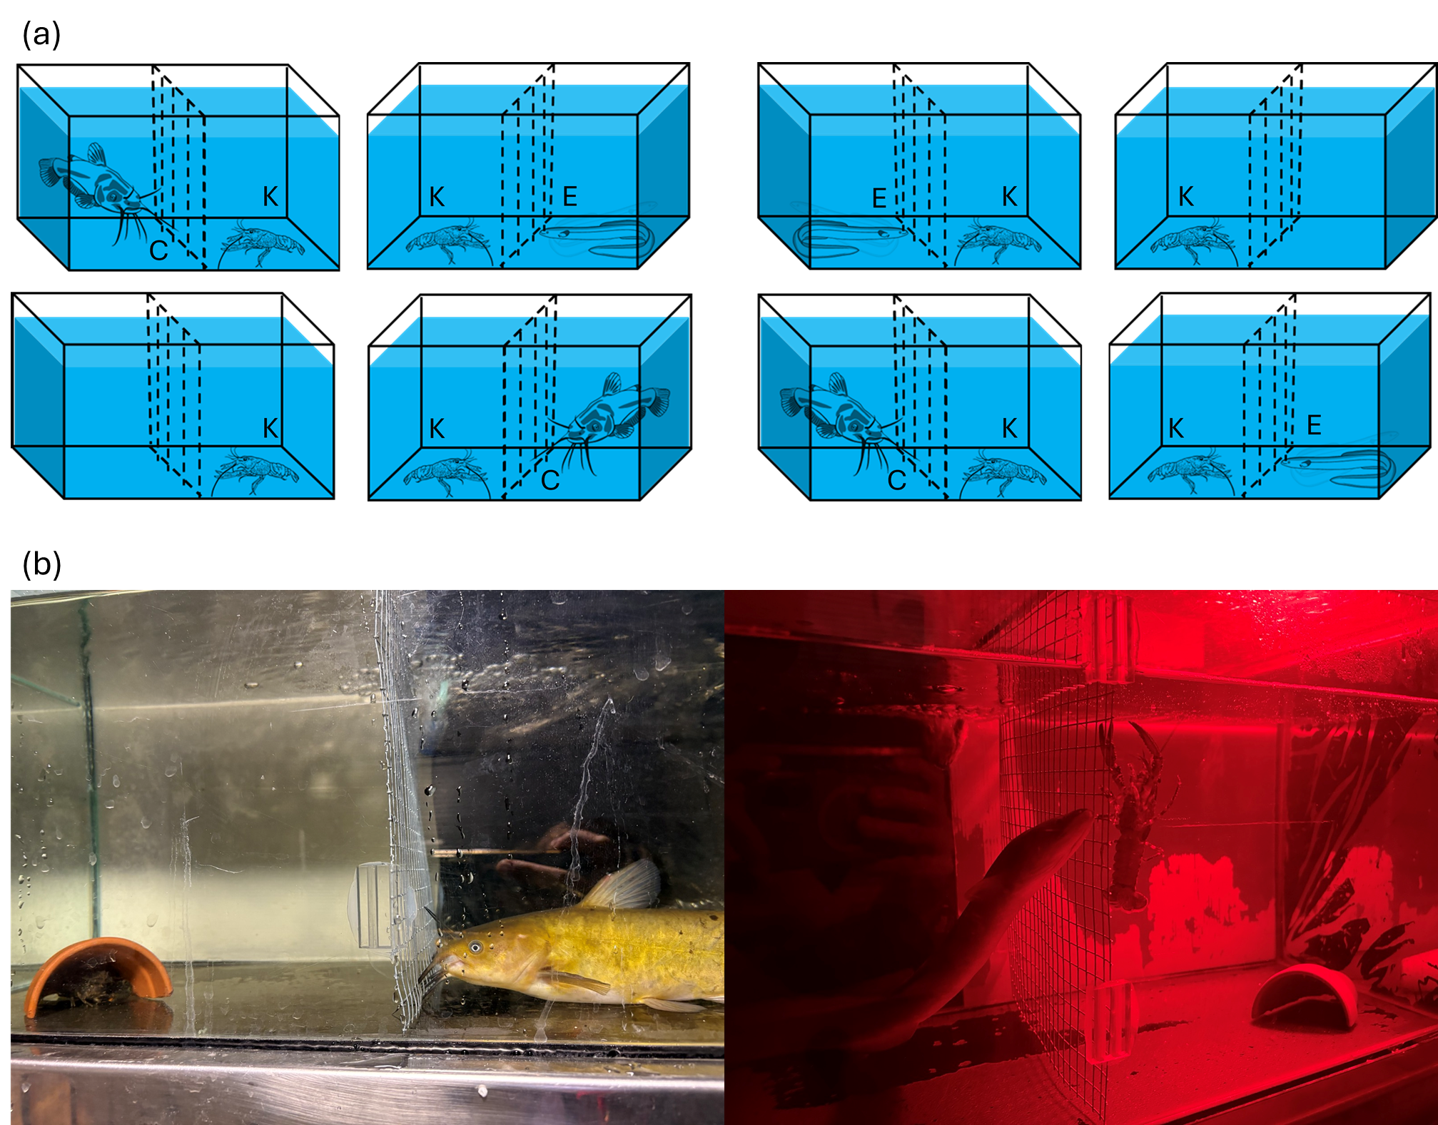
\includegraphics[keepaspectratio]{images/setup_combined.png}}

}

\caption{\label{fig-aquarium-setup}(a) Aquarium layout for kōura refuge
seeking behaviour experiment. Each experimental round consisted of eight
aquaria run simultaneously. Each tank contained a single kōura (K) and
refuge (half terracotta plant pot) on one side of a mesh divider. On the
other side was either a single catfish (C), eel (E) or a control with no
fish. The mesh divider allowed visual and chemical cues while preventing
direct physical contact between tank occupants. (b) Experiments were
repeated in light and dark (red light), with photographs showing a
catfish in the light regime (left) and and an eel in the dark regime
(red light) (right) separated from kōura by mesh dividers.}

\end{figure}%

\begin{figure}

\centering{


\includegraphics[width=6.5in,height=\textheight,keepaspectratio]{outputs/fig-emmeans-stratified.png}

}

\caption{\label{fig-emmeans-stratified}Predicted marginal probabilities
of refuge use by treatment and experimental period in light and dark
conditions. Results are shown separately for light (top) and dark
(bottom) conditions, each fitted with a beta-binomial GLMM. Points
represent model-estimated marginal means with 95\% confidence intervals
shown as error bars. Different letters (a, b) indicate statistically
significant differences based on Tukey-adjusted pairwise comparisons
within each factor. The dashed line at 0.5 marks the threshold where
kōura spend half their time in refuge.}

\end{figure}%

\begin{figure}

\centering{


\includegraphics[width=6.5in,height=\textheight,keepaspectratio]{outputs/fig-refuge-plot.png}

}

\caption{\label{fig-refuge-plot}Kōura refuge use over the course of the
experiment, showing the proportion of time spent in refuge across three
periods (before, during, and after predator exposure) for each treatment
(catfish: dark grey solid line; eel: medium grey dashed line; control:
light grey dot-dash line) under light (top) and dark (bottom)
conditions. Black dashed vertical lines indicate the start and end of
predator exposure and grey vertical lines show individual observation
times.}

\end{figure}%

\begin{figure}

\centering{

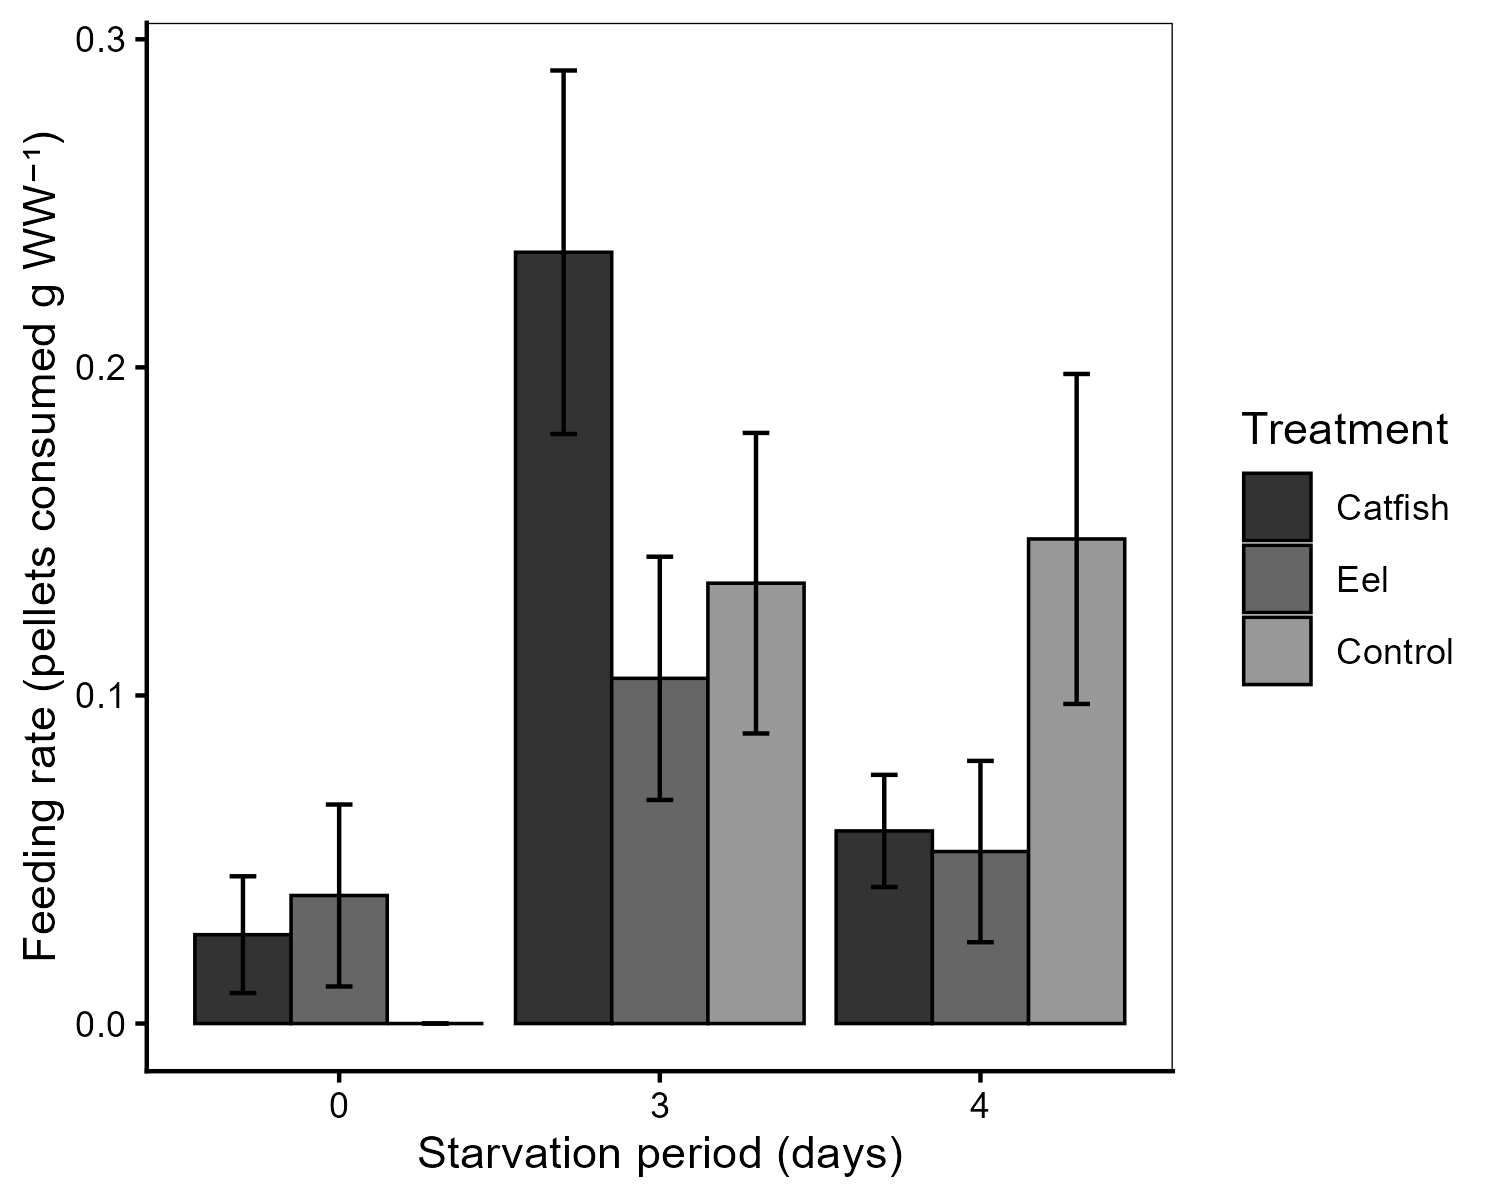
\includegraphics[width=5in,height=\textheight,keepaspectratio]{outputs/fig-feeding-plot.png}

}

\caption{\label{fig-feeding-plot}Mean (±SE) kōura feeding rate (pellets
consumed per gram wet weight kōura) across predator treatments (catfish,
eel, control) and starvation periods (0, 3, and 4 days).}

\end{figure}%

\subsection{Supplementary information}\label{supplementary-information}

\begin{longtable}[]{@{}
  >{\raggedright\arraybackslash}p{(\linewidth - 10\tabcolsep) * \real{0.1364}}
  >{\raggedright\arraybackslash}p{(\linewidth - 10\tabcolsep) * \real{0.1515}}
  >{\raggedright\arraybackslash}p{(\linewidth - 10\tabcolsep) * \real{0.1364}}
  >{\raggedleft\arraybackslash}p{(\linewidth - 10\tabcolsep) * \real{0.1212}}
  >{\raggedleft\arraybackslash}p{(\linewidth - 10\tabcolsep) * \real{0.1364}}
  >{\raggedleft\arraybackslash}p{(\linewidth - 10\tabcolsep) * \real{0.3182}}@{}}
\caption{Proportion of kōura observations recorded in refuge across
experimental treatments (catfish, eel, control), light conditions
(light, dark), and periods (before, during, and after predator
exposure). Combined rows summarise across all levels of a given factor.
Values represent the proportion of total observations where kōura were
located in the refuge.}\tabularnewline
\toprule\noalign{}
\begin{minipage}[b]{\linewidth}\raggedright
Light
\end{minipage} & \begin{minipage}[b]{\linewidth}\raggedright
Treatment
\end{minipage} & \begin{minipage}[b]{\linewidth}\raggedright
Period
\end{minipage} & \begin{minipage}[b]{\linewidth}\raggedleft
N total
\end{minipage} & \begin{minipage}[b]{\linewidth}\raggedleft
N refuge
\end{minipage} & \begin{minipage}[b]{\linewidth}\raggedleft
Proportion in refuge
\end{minipage} \\
\midrule\noalign{}
\endfirsthead
\toprule\noalign{}
\begin{minipage}[b]{\linewidth}\raggedright
Light
\end{minipage} & \begin{minipage}[b]{\linewidth}\raggedright
Treatment
\end{minipage} & \begin{minipage}[b]{\linewidth}\raggedright
Period
\end{minipage} & \begin{minipage}[b]{\linewidth}\raggedleft
N total
\end{minipage} & \begin{minipage}[b]{\linewidth}\raggedleft
N refuge
\end{minipage} & \begin{minipage}[b]{\linewidth}\raggedleft
Proportion in refuge
\end{minipage} \\
\midrule\noalign{}
\endhead
\bottomrule\noalign{}
\endlastfoot
light & catfish & before & 66 & 34 & 0.52 \\
light & catfish & during & 99 & 71 & 0.72 \\
light & catfish & after & 66 & 48 & 0.73 \\
light & eel & before & 66 & 23 & 0.35 \\
light & eel & during & 99 & 49 & 0.49 \\
light & eel & after & 66 & 35 & 0.53 \\
light & control & before & 60 & 24 & 0.40 \\
light & control & during & 90 & 48 & 0.53 \\
light & control & after & 60 & 49 & 0.82 \\
dark & catfish & before & 66 & 26 & 0.39 \\
dark & catfish & during & 99 & 47 & 0.47 \\
dark & catfish & after & 66 & 46 & 0.70 \\
dark & eel & before & 66 & 18 & 0.27 \\
dark & eel & during & 99 & 41 & 0.41 \\
dark & eel & after & 66 & 24 & 0.36 \\
dark & control & before & 60 & 22 & 0.37 \\
dark & control & during & 90 & 38 & 0.42 \\
dark & control & after & 60 & 28 & 0.47 \\
combined & catfish & before & 132 & 60 & 0.45 \\
combined & catfish & during & 198 & 118 & 0.60 \\
combined & catfish & after & 132 & 94 & 0.71 \\
combined & control & before & 120 & 46 & 0.38 \\
combined & control & during & 180 & 86 & 0.48 \\
combined & control & after & 120 & 77 & 0.64 \\
combined & eel & before & 132 & 41 & 0.31 \\
combined & eel & during & 198 & 90 & 0.45 \\
combined & eel & after & 132 & 59 & 0.45 \\
light & combined & before & 192 & 81 & 0.42 \\
light & combined & during & 288 & 168 & 0.58 \\
light & combined & after & 192 & 132 & 0.69 \\
dark & combined & before & 192 & 66 & 0.34 \\
dark & combined & during & 288 & 126 & 0.44 \\
dark & combined & after & 192 & 98 & 0.51 \\
combined & combined & before & 384 & 147 & 0.38 \\
combined & combined & during & 576 & 294 & 0.51 \\
combined & combined & after & 384 & 230 & 0.60 \\
combined & combined & combined & 1344 & 671 & 0.50 \\
\end{longtable}

{

\begin{longtable}[]{@{}lrrrrr@{}}

\caption{\label{tbl-feeding-summary}Fixed effects from the linear mixed
model of kōura feeding rate (pellets consumed per gram body weight).
Starvation period included as fixed effect with tank as random
intercept.}

\tabularnewline

\toprule\noalign{}
Term & Estimate & Std. Error & df & t value & p value \\
\midrule\noalign{}
\endhead
\bottomrule\noalign{}
\endlastfoot
(Intercept) & 0.023 & 0.024 & 43 & 0.951 & 0.347 \\
day\_starve3 & 0.132 & 0.033 & 43 & 4.033 & 0.000 \\
day\_starve4 & 0.067 & 0.033 & 43 & 2.056 & 0.046 \\

\end{longtable}

}

\textsubscript{Source:
\href{https://OlivierRaven.github.io/https---github.com-OlivierRaven-NCE_Koura_catfish/analysis-preview.html\#cell-tbl-feeding-summary}{Analysis
Notebook}}

\protect\phantomsection\label{refs}
\begin{CSLReferences}{1}{1}
\bibitem[\citeproctext]{ref-Abrams2000}
Abrams PA (2000) The evolution of predator-prey interactions: Theory and
evidence. Annual Review of Ecology and Systematics 31:79--105.
\url{https://doi.org/10.1146/annurev.ecolsys.31.1.79}

\bibitem[\citeproctext]{ref-Achtymichuk2025}
Achtymichuk GH, Fish KM, Ferrari MCO (2025) The power of concentration:
Antipredator responses to diluted frozen crayfish alarm cues provide
insights on ecologically relevant concentrations and updates to
methodology. PLOS One 20:e0340001.
\url{https://doi.org/10.1371/journal.pone.0340001}

\bibitem[\citeproctext]{ref-Adams2007}
Adams SB (2007) Direct and indirect effects of channel catfish
({\emph{Ictalurus punctatus}}) on native crayfishes ({Cambaridae}) in
experimental tanks. The American Midland Naturalist 158:85--96.
\url{https://doi.org/10.1674/0003-0031(2007)158\%5B85:daieoc\%5D2.0.co;2}

\bibitem[\citeproctext]{ref-Appelberg1993}
Appelberg M, Soederbaeck B, Odelstroem T (1993) Predator detection and
perception of predation risk in the crayfish {\emph{Astacus astacus}} l.
Nordic journal of freshwater research 68:55--62

\bibitem[\citeproctext]{ref-Barnes2003}
Barnes GE, Hicks BJ (2003) Brown bullhead catfish ({\emph{Ameiurus
nebulosus}}) in {Lake Taupo}. In: Managing invasive freshwater fish in
{New Zealand}: Proceedings of a workshop hosted by {Department of
Conservation}, 10-12 may 2001, {Hamilton}. Department of Conservation

\bibitem[\citeproctext]{ref-Beattie2018}
Beattie MC, Moore PA (2018) Predator recognition of chemical cues in
crayfish: Diet~and experience influence the ability
to~detect~predation~threats. Behaviour 155:505--530.
\url{https://doi.org/10.1163/1568539x-00003501}

\bibitem[\citeproctext]{ref-Blake1993}
Blake MA, Hart PJB (1993) The behavioural responses of juvenile signal
crayfish {\emph{Pacifastacus leniusculus}} to stimuli from perch and
eels. Freshwater Biology 29:89--97.
\url{https://doi.org/10.1111/j.1365-2427.1993.tb00747.x}

\bibitem[\citeproctext]{ref-Bronmark2012}
Brönmark C, Hansson L-A (2012) Chemical ecology in aquatic systems.
Oxford University Press

\bibitem[\citeproctext]{ref-Brooks2017}
Brooks M, Bolker B, Kristensen K, et al (2017)
\href{https://doi.org/10.32614/cran.package.glmmtmb}{glmmTMB:
Generalized linear mixed models using template model builder}. CRAN:
Contributed Packages

\bibitem[\citeproctext]{ref-Brown2004}
Brown GE, Poirier J-F, Adrian JC (2004) Assessment of local predation
risk: The role of subthreshold concentrations of chemical alarm cues.
Behavioral Ecology 15:810--815.
\url{https://doi.org/10.1093/beheco/arh084}

\bibitem[\citeproctext]{ref-Brown2009}
Brown LA (2009) \href{http://hdl.handle.net/10179/1168}{Habitat
determinants and predatory interactions of the endemic freshwater
crayfish (koura, {\emph{Paranephrops planifrons}}) in the lower {North
Island}, {New Zealand}}. Master's thesis, Massey University

\bibitem[\citeproctext]{ref-Carthey2014}
Carthey AJR, Banks PB (2014) Naïveté in novel ecological interactions:
Lessons from theory and experimental evidence. Biological Reviews
89:932--949. \url{https://doi.org/10.1111/brv.12087}

\bibitem[\citeproctext]{ref-Clinchy2013}
Clinchy M, Sheriff MJ, Zanette LY (2012) Predator‐induced stress and the
ecology of fear. Functional Ecology 27:56--65.
\url{https://doi.org/10.1111/1365-2435.12007}

\bibitem[\citeproctext]{ref-Collier1997}
Collier KJ, Parkyn SM, Rabeni CF (1997) Koura: A keystone species. Water
and Atmosphere 5:18--20

\bibitem[\citeproctext]{ref-Dawkins1979}
Dawkins R, Krebs JR (1979) Arms races between and within species.
Proceedings of the Royal Society of London B Biological Sciences
205:489--511. \url{https://doi.org/10.1098/rspb.1979.0081}

\bibitem[\citeproctext]{ref-Dedual2019}
Dedual M (2019)
\href{https://atlas.boprc.govt.nz/api/v1/edms/document/A3591759/content}{Summary
of the impacts and control methods of {Brown Bullhead} catfish
({\emph{Ameiurus nebulosus}} {Lesueur} 1815) in {New Zealand} and
overseas}. {Bay of Plenty} Regional Council

\bibitem[\citeproctext]{ref-Devcich1979}
Devcich AA (1979) An ecological study of {\emph{Paranephrops
planifrons}} {White} ({Decapoda}: {Parastacidae}) in {Lake Rotoiti},
{North Island}. PhD thesis, University of Waikato

\bibitem[\citeproctext]{ref-Doherty2016}
Doherty TS, Glen AS, Nimmo DG, et al (2016) Invasive predators and
global biodiversity loss. Proceedings of the National Academy of
Sciences 113:11261--11265. \url{https://doi.org/10.1073/pnas.1602480113}

\bibitem[\citeproctext]{ref-Driscoll2020}
Driscoll J, Kola M, Mathews L (2020) Perception of alarm cues influences
the outcome of shelter competition in crayfish20. Ethology 126:584--592.
\url{https://doi.org/10.1111/eth.13011}

\bibitem[\citeproctext]{ref-Ehlman2019}
Ehlman SM, Trimmer PC, Sih A (2019) Prey responses to exotic predators:
Effects of old risks and new cues. The American Naturalist 193:575--587.
\url{https://doi.org/10.1086/702252}

\bibitem[\citeproctext]{ref-Feldmann1994}
Feldmann RM, Pole M (1994) A new species of {\emph{Paranephrops}}
{White}, 1842: A fossil freshwater crayfish ({Decapoda}: {Parastacidae})
from the {Manuherikia Group} ({Miocene}), {Central Otago}, {New
Zealand}. New Zealand Journal of Geology and Geophysics 37:163--167.
\url{https://doi.org/10.1080/00288306.1994.9514611}

\bibitem[\citeproctext]{ref-Figler2005}
Figler MH, Blank GS, Peeke HVS (2005) Shelter competition between
resident male red swamp crayfish {\emph{Procambarus clarkii}} ({Girard})
and conspecific intruders varying by sex and reproductive status. Marine
and Freshwater Behaviour and Physiology 38:237--248.
\url{https://doi.org/10.1080/10236240500376477}

\bibitem[\citeproctext]{ref-Francis2019}
Francis LB (2019)
\href{https://researchcommons.waikato.ac.nz/handle/10289/12746}{Evaluating
the effects of invasive brown bullhead catfish ({\emph{Ameiurus
nebulosus}}) on k{ō}ura (freshwater crayfish, {\emph{Paranephrops
planifrons}}) in {Lake Rotoiti}}. Master's thesis, University of Waikato

\bibitem[\citeproctext]{ref-Gherardi2011}
Gherardi F, Mavuti KM, Pacini N, et al (2011) The smell of danger:
Chemical recognition of fish predators by the invasive crayfish
{\emph{Procambarus clarkii}}. Freshwater Biology 56:1567--1578.
\url{https://doi.org/10.1111/j.1365-2427.2011.02595.x}

\bibitem[\citeproctext]{ref-Hartig2024}
{Hartig F, Lohse L, leite M de S} (2024)
\href{https://cran.r-project.org/web/packages/DHARMa/index.html}{DHARMa:
Residual diagnostics for hierarchical (multi-level / mixed) regression
models}

\bibitem[\citeproctext]{ref-Hazlett2003}
Hazlett BA (2003) The effects of starvation on crayfish responses to
alarm odor. Ethology 109:587--592.
\url{https://doi.org/10.1046/j.1439-0310.2003.00902.x}

\bibitem[\citeproctext]{ref-Hicks1997}
Hicks BJ (1997) Food webs in forest and pasture streams in the {Waikato}
region, {New Zealand}: A study based on analyses of stable isotopes of
carbon and nitrogen, and fish gut contents. New Zealand Journal of
Marine and Freshwater Research 31:651--664.
\url{https://doi.org/10.1080/00288330.1997.9516796}

\bibitem[\citeproctext]{ref-Hogg2003}
Hogg AG, Higham TFG, Lowe DJ, et al (2003) A wiggle-match date for
{Polynesian} settlement of {New Zealand}. Antiquity 77:116--125.
\url{https://doi.org/10.1017/s0003598x00061408}

\bibitem[\citeproctext]{ref-Johnson2014}
Johnson MF, Rice SP, Reid I (2014) The activity of signal crayfish
({\emph{Pacifastacus leniusculus}}) in relation to thermal and hydraulic
dynamics of an alluvial stream, {UK}. Hydrobiologia 724:41--54.
\url{https://doi.org/10.1007/s10750-013-1708-1}

\bibitem[\citeproctext]{ref-Kasumyan2022}
Kasumyan AO (2022) Fish as sources of kairomones-chemical signals for
aquatic animals. Journal of Ichthyology 62:289--315.
\url{https://doi.org/10.1134/s0032945222020084}

\bibitem[\citeproctext]{ref-Kaulfuss2018}
Kaulfuss U, Lee DE, Wartho J-A, et al (2018) Geology and palaeontology
of the {Hindon Maar Complex}: A {Miocene} terrestrial fossil
{\emph{Lagerstätte}} in southern {New Zealand}. Palaeogeography,
Palaeoclimatology, Palaeoecology 500:52--68.
\url{https://doi.org/10.1016/j.palaeo.2018.03.022}

\bibitem[\citeproctext]{ref-Kindlinger2017}
Kindinger TL, Albins MA (2017) Consumptive and non-consumptive effects
of an invasive marine predator on native coral-reef herbivores.
Biological Invasions 19:131--146.
\url{https://doi.org/10.1007/s10530-016-1268-1}

\bibitem[\citeproctext]{ref-Kusabs2026}
Kusabs IAK, Duggan IC, Bruere AC, et al (2026) Invasive catfish linked
to the decline of freshwater crayfish in two {Aotearoa New Zealand}
lakes. Biological Invasions 28:
\url{https://doi.org/10.1007/s10530-026-03852-0}

\bibitem[\citeproctext]{ref-Kusabs2009}
Kusabs IA, Quinn JM (2009) Use of a traditional {Māori} harvesting
method, the tau kōura, for monitoring kōura (freshwater crayfish,
{\emph{Paranephrops planifrons}}) in {Lake Rotoiti}, {North Island},
{New Zealand}. New Zealand Journal of Marine and Freshwater Research
43:713--722. \url{https://doi.org/10.1080/00288330909510036}

\bibitem[\citeproctext]{ref-Laundre2001}
Laundré JW, Hernández L, Altendorf KB (2001) Wolves, elk, and bison:
Reestablishing the {``landscape of fear''} in {Yellowstone National
Park}, {U.S.A.} Canadian Journal of Zoology 79:1401--1409.
\url{https://doi.org/10.1139/z01-094}

\bibitem[\citeproctext]{ref-Lee2025}
Lee F, Kusabs IAK, Perry GLW, MacNeil C (2025) Identifying refugia from
the synergistic threats of climate change and invasive species. Web
Ecology 25:221--239. \url{https://doi.org/10.5194/we-25-221-2025}

\bibitem[\citeproctext]{ref-Lenth2026}
Lenth RV, Piaskowski J, Banfai B, et al (2026)
\href{https://cran.r-project.org/web/packages/emmeans/index.html}{{emmeans}:
Estimated marginal means, aka least-squares means}

\bibitem[\citeproctext]{ref-Lima1990}
Lima SL, Dill LM (1990) Behavioral decisions made under the risk of
predation: A review and prospectus. Canadian Journal of Zoology
68:619--640. \url{https://doi.org/10.1139/z90-092}

\bibitem[\citeproctext]{ref-MacNeil2025}
MacNeil C, Lee F, Kusabs I, Holmes R (2025) The biter bit; scavenging
behaviour of native freshwater crayfish on the carrion of native and
introduced fish predators in {Aotearoa-New Zealand}. Knowledge \&
Management of Aquatic Ecosystems 29.
\url{https://doi.org/10.1051/kmae/2025022}

\bibitem[\citeproctext]{ref-Martin2014}
Martin CW (2014) Naïve prey exhibit reduced antipredator behavior and
survivorship. PeerJ 2:e665. \url{https://doi.org/10.7717/peerj.665}

\bibitem[\citeproctext]{ref-Martin2007}
Martin M, Boubée J, Kusabs I (2007)
\href{https://niwa.co.nz/sites/default/files/2025-04/te_arawa_species_report_tuna_0.pdf}{Taonga
and mahinga kai of the {Te Arawa} lakes: A review of current knowledge -
tuna}. {National Institute of Water} \& {Atmospheric Research Ltd},
{Hamilton}, {New Zealand}

\bibitem[\citeproctext]{ref-McDowall1990}
McDowall RM (1990)
\href{https://agris.fao.org/search/en/providers/122621/records/6473966cce9437aa76003d0e}{{New
Zealand} freshwater fishes: A natural history and guide}

\bibitem[\citeproctext]{ref-Nystrom2005}
Nyström P (2005) Non‐lethal predator effects on the performance of a
native and an exotic crayfish species. Freshwater Biology 50:1938--1949.
\url{https://doi.org/10.1111/j.1365-2427.2005.01438.x}

\bibitem[\citeproctext]{ref-Parkyn2001}
Parkyn SM, Collier KJ, Hicks BJ (2001) {New Zealand} stream crayfish:
Functional omnivores but trophic predators? Freshwater Biology
46:641--652. \url{https://doi.org/10.1046/j.1365-2427.2001.00702.x}

\bibitem[\citeproctext]{ref-Peacor2001}
Peacor SD, Werner EE (2001) The contribution of trait-mediated indirect
effects to the net effects of a predator. Proceedings of the National
Academy of Sciences 98:3904--3908.
\url{https://doi.org/10.1073/pnas.071061998}

\bibitem[\citeproctext]{ref-Preisser2005}
Preisser EL, Bolnick DI, Benard MF (2005) Scared to death? The effects
of intimidation and consumption in predator-prey interactions. Ecology
86:501--509. \url{https://doi.org/10.1890/04-0719}

\bibitem[\citeproctext]{ref-RCoreTeam2025}
R Core Team (2025) \href{https://www.R-project.org/}{{R}: A language and
environment for statistical computing}. R Foundation for Statistical
Computing, Vienna, Austria

\bibitem[\citeproctext]{ref-RambergPihl2020}
Ramberg-Pihl NC, Yurewicz KL (2020) Behavioral responses of northern
crayfish ({\emph{Faxonius virilis}}) to conspecific alarm cues and
predator cues from smallmouth bass ({\emph{Micropterus dolomieu}}).
Marine and Freshwater Behaviour and Physiology 53:1--16.
\url{https://doi.org/10.1080/10236244.2020.1717338}

\bibitem[\citeproctext]{ref-Ryan2009}
Ryan P (2009) \href{https://teara.govt.nz/en/eels}{Eels \textbar{} {Te
Ara Encyclopedia of New Zealand}}

\bibitem[\citeproctext]{ref-Schmitz1997}
Schmitz OJ, Beckerman AP, O'Brien KM (1997) Behaviorally mediated
trophic cascades: Effects of predation risk on food web interactions.
Ecology 78:1388--1399.
\url{https://doi.org/10.1890/0012-9658(1997)078\%5B1388:bmtceo\%5D2.0.co;2}

\bibitem[\citeproctext]{ref-Scott1973}
Scott WB, Crossman EJ (1973) Freshwater fishes of {Canada}. Fisheries
Research Board of Canada

\bibitem[\citeproctext]{ref-Shave1994}
Shave CathyR, Townsend CR, Crowl TA (1994) Anti-predator behaviours of a
freshwater crayfish ({\emph{Paranephrops zealandicus}}) to a native and
an introduced predator. New Zealand Journal of Ecology 18:1--10

\bibitem[\citeproctext]{ref-Sheriff2020}
Sheriff MJ, Peacor SD, Hawlena D, Thaker M (2020) Non-consumptive
predator effects on prey population size: A dearth of evidence. Journal
of Animal Ecology 89:1302--1316.
\url{https://doi.org/10.1111/1365-2656.13213}

\bibitem[\citeproctext]{ref-Sih2010}
Sih A, Bolnick DI, Luttbeg B, et al (2010) Predator-prey naïveté,
antipredator behavior, and the ecology of predator invasions. Oikos
119:610--621. \url{https://doi.org/10.1111/j.1600-0706.2009.18039.x}

\bibitem[\citeproctext]{ref-Sih2023}
Sih A, Chung HJ, Neylan I, et al (2023) Fear generalization and
behavioral responses to multiple dangers. Trends in Ecology \& Evolution
38:369--380. \url{https://doi.org/10.1016/j.tree.2022.11.001}

\bibitem[\citeproctext]{ref-Sih2011}
Sih A, Ferrari MCO, Harris DJ (2011) Evolution and behavioural responses
to human‐induced rapid environmental change. Evolutionary Applications
4:367--387. \url{https://doi.org/10.1111/j.1752-4571.2010.00166.x}

\bibitem[\citeproctext]{ref-Smee2006}
Smee DL, Weissburg MJ (2006) Hard clams ({\emph{Mercenaria mercenaria}})
evaluate predation risk using chemical signals from predators and
injured conspecifics. Journal of Chemical Ecology 32:605--619.
\url{https://doi.org/10.1007/s10886-005-9021-8}

\bibitem[\citeproctext]{ref-Sniegula2025}
Sniegula S, Konczarek D, Bonk M, et al (2025) Non-consumptive effects of
native, alien and invasive alien crayfish on damselfly egg life history
and carry-over effects on larval physiology. NeoBiota 97:215--235.
\url{https://doi.org/10.3897/neobiota.97.139760}

\bibitem[\citeproctext]{ref-Stebbing2010}
Stebbing PD, Watson GJ, Bentley MG (2010) The response to disturbance
chemicals and predator odours of juvenile and adult signal crayfish
{\emph{Pacifastacus leniusculus}} ({Dana}). Marine and Freshwater
Behaviour and Physiology 43:183--195.
\url{https://doi.org/10.1080/10236244.2010.487301}

\bibitem[\citeproctext]{ref-Stein1976}
Stein RA, Magnuson JJ (1976) Behavioral response of crayfish to a fish
predator. Ecology 57:751--761. \url{https://doi.org/10.2307/1936188}

\bibitem[\citeproctext]{ref-Usio2004}
Usio N, Townsend CR (2004) Roles of crayfish: Consequences of predation
and bioturbation for stream invertebrates. Ecology 85:807--822.
\url{https://doi.org/10.1890/02-0618}

\bibitem[\citeproctext]{ref-Wood2020a}
Wood TC, Moore PA (2020b) Big and bad: How relative predator size and
dietary information influence rusty crayfish ({\emph{Faxonius
rusticus}}) behavior and resource-use decisions. Canadian Journal of
Zoology 98:62--72. \url{https://doi.org/10.1139/cjz-2019-0089}

\bibitem[\citeproctext]{ref-Wood2020b}
Wood TC, Moore PA (2020a) Fine-tuned responses to chemical landscapes:
Crayfish use predator odors to assess threats based on relative size
ratios. Ecosphere 11:e03188. \url{https://doi.org/10.1002/ecs2.3188}

\bibitem[\citeproctext]{ref-Wright2010}
Wright TF, Eberhard JR, Hobson EA, et al (2010) Behavioral flexibility
and species invasions: The adaptive flexibility hypothesis. Ethology
Ecology \& Evolution 22:393--404.
\url{https://doi.org/10.1080/03949370.2010.505580}

\bibitem[\citeproctext]{ref-Zhao2024}
Zhao M, Feng G, Wang H, et al (2024) The influence of shelter type and
coverage on crayfish ({\emph{Procambarus clarkii}}) predation by catfish
({\emph{Silurus asotus}}): A controlled environment study. Animals
14:1147. \url{https://doi.org/10.3390/ani14081147}

\end{CSLReferences}




\end{document}
